\documentclass[
  man,
  longtable,
  nolmodern,
  notxfonts,
  notimes,
  colorlinks=true,linkcolor=blue,citecolor=blue,urlcolor=blue]{apa7}

\usepackage{amsmath}
\usepackage{amssymb}




\RequirePackage{longtable}
\RequirePackage{threeparttablex}

\makeatletter
\renewcommand{\paragraph}{\@startsection{paragraph}{4}{\parindent}%
	{0\baselineskip \@plus 0.2ex \@minus 0.2ex}%
	{-.5em}%
	{\normalfont\normalsize\bfseries\typesectitle}}

\renewcommand{\subparagraph}[1]{\@startsection{subparagraph}{5}{0.5em}%
	{0\baselineskip \@plus 0.2ex \@minus 0.2ex}%
	{-\z@\relax}%
	{\normalfont\normalsize\bfseries\itshape\hspace{\parindent}{#1}\textit{\addperi}}{\relax}}
\makeatother




\usepackage{longtable, booktabs, multirow, multicol, colortbl, hhline, caption, array, float, xpatch}
\setcounter{topnumber}{2}
\setcounter{bottomnumber}{2}
\setcounter{totalnumber}{4}
\renewcommand{\topfraction}{0.85}
\renewcommand{\bottomfraction}{0.85}
\renewcommand{\textfraction}{0.15}
\renewcommand{\floatpagefraction}{0.7}

\usepackage{tcolorbox}
\tcbuselibrary{listings,theorems, breakable, skins}
\usepackage{fontawesome5}

\definecolor{quarto-callout-color}{HTML}{909090}
\definecolor{quarto-callout-note-color}{HTML}{0758E5}
\definecolor{quarto-callout-important-color}{HTML}{CC1914}
\definecolor{quarto-callout-warning-color}{HTML}{EB9113}
\definecolor{quarto-callout-tip-color}{HTML}{00A047}
\definecolor{quarto-callout-caution-color}{HTML}{FC5300}
\definecolor{quarto-callout-color-frame}{HTML}{ACACAC}
\definecolor{quarto-callout-note-color-frame}{HTML}{4582EC}
\definecolor{quarto-callout-important-color-frame}{HTML}{D9534F}
\definecolor{quarto-callout-warning-color-frame}{HTML}{F0AD4E}
\definecolor{quarto-callout-tip-color-frame}{HTML}{02B875}
\definecolor{quarto-callout-caution-color-frame}{HTML}{FD7E14}

\newlength\Oldarrayrulewidth
\newlength\Oldtabcolsep


\usepackage{hyperref}




\providecommand{\tightlist}{%
  \setlength{\itemsep}{0pt}\setlength{\parskip}{0pt}}
\usepackage{longtable,booktabs,array}
\usepackage{calc} % for calculating minipage widths
% Correct order of tables after \paragraph or \subparagraph
\usepackage{etoolbox}
\makeatletter
\patchcmd\longtable{\par}{\if@noskipsec\mbox{}\fi\par}{}{}
\makeatother
% Allow footnotes in longtable head/foot
\IfFileExists{footnotehyper.sty}{\usepackage{footnotehyper}}{\usepackage{footnote}}
\makesavenoteenv{longtable}

\usepackage{graphicx}
\makeatletter
\def\maxwidth{\ifdim\Gin@nat@width>\linewidth\linewidth\else\Gin@nat@width\fi}
\def\maxheight{\ifdim\Gin@nat@height>\textheight\textheight\else\Gin@nat@height\fi}
\makeatother
% Scale images if necessary, so that they will not overflow the page
% margins by default, and it is still possible to overwrite the defaults
% using explicit options in \includegraphics[width, height, ...]{}
\setkeys{Gin}{width=\maxwidth,height=\maxheight,keepaspectratio}
% Set default figure placement to htbp
\makeatletter
\def\fps@figure{htbp}
\makeatother


% definitions for citeproc citations
\NewDocumentCommand\citeproctext{}{}
\NewDocumentCommand\citeproc{mm}{%
  \begingroup\def\citeproctext{#2}\cite{#1}\endgroup}
\makeatletter
 % allow citations to break across lines
 \let\@cite@ofmt\@firstofone
 % avoid brackets around text for \cite:
 \def\@biblabel#1{}
 \def\@cite#1#2{{#1\if@tempswa , #2\fi}}
\makeatother
\newlength{\cslhangindent}
\setlength{\cslhangindent}{1.5em}
\newlength{\csllabelwidth}
\setlength{\csllabelwidth}{3em}
\newenvironment{CSLReferences}[2] % #1 hanging-indent, #2 entry-spacing
 {\begin{list}{}{%
  \setlength{\itemindent}{0pt}
  \setlength{\leftmargin}{0pt}
  \setlength{\parsep}{0pt}
  % turn on hanging indent if param 1 is 1
  \ifodd #1
   \setlength{\leftmargin}{\cslhangindent}
   \setlength{\itemindent}{-1\cslhangindent}
  \fi
  % set entry spacing
  \setlength{\itemsep}{#2\baselineskip}}}
 {\end{list}}
\usepackage{calc}
\newcommand{\CSLBlock}[1]{\hfill\break\parbox[t]{\linewidth}{\strut\ignorespaces#1\strut}}
\newcommand{\CSLLeftMargin}[1]{\parbox[t]{\csllabelwidth}{\strut#1\strut}}
\newcommand{\CSLRightInline}[1]{\parbox[t]{\linewidth - \csllabelwidth}{\strut#1\strut}}
\newcommand{\CSLIndent}[1]{\hspace{\cslhangindent}#1}





\usepackage{newtx}

\defaultfontfeatures{Scale=MatchLowercase}
\defaultfontfeatures[\rmfamily]{Ligatures=TeX,Scale=1}





\title{Removing the disguise: the matched guise technique and listener
awareness}


\shorttitle{Removing the disguise: the matched guise technique and
listener awareness}


\usepackage{etoolbox}









\authorsnames[{1},{2}]{Kyler Laycock,Kevin B McGowan}







\authorsaffiliations{
{The Ohio State University},{The University of Kentucky}}




\leftheader{Laycock and McGowan}

\date{2024-05-21}


\abstract{Sociophonetic perception is often studied using versions of
the matched guise technique. Linguists using this technique appear
united in the methodological assumptions that participants believe the
manipulation and that this belief influences perception below the level
of introspective awareness. We report an audiovisual matched guise
experiment with a novel `unhidden' instruction condition. The basic task
is a replication of the Strand effect (\citeproc{ref-strand1999}{Strand,
1999}; \citeproc{ref-strandJohnson1996}{Strand \& Johnson, 1996}).
Participants in the `unhidden' condition were instructed that the man or
woman in the photo did not represent the voice they were listening to.
Participants in both guises exhibited the Strand effect to nearly
numerically identical extents. This result suggests that participants
need not believe a link exists between a voice and a purported social
category for visually-cued social information to influence segmental
perception. We explore the implications of this result for the MGT and
for theories of social awareness and speech perception more broadly.}



\authornote{\par{\addORCIDlink{Kyler
Laycock}{0000-0002-3731-0841}}\par{\addORCIDlink{Kevin B
McGowan}{0000-0002-8214-1901}} 

\par{       }
\par{Correspondence concerning this article should be addressed to Kyler
Laycock, Email: laycock.21@buckeyemail.osu.edu}
}

\makeatletter
\let\endoldlt\endlongtable
\def\endlongtable{
\hline
\endoldlt
}
\makeatother
\RequirePackage{longtable}
\DeclareDelayedFloatFlavor{longtable}{table}

\urlstyle{same}



\makeatletter
\@ifpackageloaded{caption}{}{\usepackage{caption}}
\AtBeginDocument{%
\ifdefined\contentsname
  \renewcommand*\contentsname{Table of contents}
\else
  \newcommand\contentsname{Table of contents}
\fi
\ifdefined\listfigurename
  \renewcommand*\listfigurename{List of Figures}
\else
  \newcommand\listfigurename{List of Figures}
\fi
\ifdefined\listtablename
  \renewcommand*\listtablename{List of Tables}
\else
  \newcommand\listtablename{List of Tables}
\fi
\ifdefined\figurename
  \renewcommand*\figurename{Figure}
\else
  \newcommand\figurename{Figure}
\fi
\ifdefined\tablename
  \renewcommand*\tablename{Table}
\else
  \newcommand\tablename{Table}
\fi
}
\@ifpackageloaded{float}{}{\usepackage{float}}
\floatstyle{ruled}
\@ifundefined{c@chapter}{\newfloat{codelisting}{h}{lop}}{\newfloat{codelisting}{h}{lop}[chapter]}
\floatname{codelisting}{Listing}
\newcommand*\listoflistings{\listof{codelisting}{List of Listings}}
\makeatother
\makeatletter
\makeatother
\makeatletter
\@ifpackageloaded{caption}{}{\usepackage{caption}}
\@ifpackageloaded{subcaption}{}{\usepackage{subcaption}}
\makeatother

% From https://tex.stackexchange.com/a/645996/211326
%%% apa7 doesn't want to add appendix section titles in the toc
%%% let's make it do it
\makeatletter
\xpatchcmd{\appendix}
  {\par}
  {\addcontentsline{toc}{section}{\@currentlabelname}\par}
  {}{}
\makeatother

\begin{document}

\maketitle


\setcounter{secnumdepth}{-\maxdimen} % remove section numbering

\setlength\LTleft{0pt}


\section{Introduction}\label{introduction}

A great deal of attention has been paid in the phonetics and
sociophonetics literatures to the perception of the voiceless fricatives
{[}ʃ{]} and {[}s{]} in English. To a first approximation, these
fricatives differ in the distance between the point of lingual
articulation and the teeth, which give them their characteristic
sibilance Shadle (\citeproc{ref-shadle1991}{1991}). English {[}s{]} has
a short resonating chamber behind the teeth; it is typically produced by
holding the tongue blade near enough to the alveolar ridge to cause
turbulent airflow. English {[}ʃ{]} has a comparatively larger resonating
chamber; it is typically produced with a more posterior, palato-alveolar
tongue position and lip rounding both of which serve to reinforce this
posteriority. But listeners do not perceive via \{++this type
of++\}\{\textgreater\textgreater KM\textless\textless\} first
approximation\{++; we are sensitive to fine phonetic details far beyond
these gross, categorical,
differences++\}\{\textgreater\textgreater KM\textless\textless\}.
Indeed, these two fricatives have been exciting to researchers precisely
because of the sensitivity listeners bring to their perception and how
that perception interacts with both linguistic and social knowledge.

\subsection{Coarticulatory and Social Information Influence
{[}ʃ{]}-{[}s{]}
perception}\label{coarticulatory-and-social-information-influence-ux283-s-perception}

\{\textgreater\textgreater KL: ok, this is the specific section the
editors didn't like I think vis-a-vis ``rewriting the introduction to
state more strongly why this study is important to sociolinguistics, and
not mainly interesting to cognitive linguists''\textless\textless\}
Listeners are sensitive to articulatory mismatches between the
fricatives {[}ʃ{]}-{[}s{]} and neighboring sounds. Whalen
(\citeproc{ref-whalen1984}{1984}) conducted a series of experiments to
investigate listeners' responses to articulatory mismatches in synthetic
speech. Overall, the result of these investigations was that
subcategorical phonetic mismatches slow phonetic judgments. In onset
position, in isolation, or in coda position, misleading coarticulatory
information inhibited reaction times. Listeners, Whalen cautions in the
conclusion, are sensitive to articulatory patterns that are below the
level of conscious awareness and not available to direct experimenter
scrutiny. While listeners will readily fill-in missing or ambiguous
information, the presence of actively \emph{conflicting} articulatory
information is inhibitory.

A commonly used methodology involves the creation of synthetic fricative
continua. These continua have endpoints in prototypical examples of
{[}ʃ{]} and {[}s{]} with some number of equal-sized acoustic steps
generated, synthesized, or even mixed between these. Somewhere in the
middle of such a continuum will be fricative-like noise that is
ambiguous as to category membership: not clearly a {[}ʃ{]} and not
clearly an {[}s{]}. \cite{May1976} paired a continuum from {[}ʃ{]} (2.9
kHz) to {[}s{]} (4.4 kHz) with synthetic {[}æ{]} vowels to form CV
pairs. May found that listeners perceived a higher proportion of the
fricative continuum as {[}ʃ{]} when paired with vowel stimuli from a
smaller vocal tract. The logic here is that smaller resonating chambers
between the lingual articulation and teeth will have a higher mean
frequency than larger resonating chambers. Listeners' use of apparent
vocal tract size in perception reflect their knowledge of this variation
(\citeproc{ref-munson2011}{Munson, 2011}).

Mann and Repp (\citeproc{ref-MannRepp1980}{1980}) replicated this
finding, extending it to natural productions of vowels spoken by a male
or female-identified talker. Similar to May's results with simulated
vocal tract size, Mann \& Repp found a higher proportion of the
fricative continuum was heard as {[}ʃ{]} when paired with the speech of
the female talker. This early work, like others of the period
(\citeproc{ref-ohala1984}{Ohala, 1984}), theorized size as being a
relatively deterministic feature of talker sexual dimorphism. One
consequence of this view is that gender-related variation in the speech
signal is considered mechanistic, universal, and following from purely
physical laws. Vocal tract size is presumably not available for
individual performance and so listener knowledge of this variation can
be correspondingly simple. Vocal tract size may influence perception,
but it does so implicitly, automatically, and below the level of
introspective awareness.

\{++ Mann and Repp (\citeproc{ref-MannRepp1980}{1980}) also replicated
and extended previous work (\citeproc{ref-kunisakifujisaki1977}{Kunisaki
\& Fujisaki, 1977}; \citeproc{ref-whalen1981}{Whalen, 1981})
demonstrating that listeners report hearing more of the synthetic
fricative continuum as {[}s{]} when followed by a rounded vowel quality
such as English {[}u{]} than when followed by an unrounded quality such
as {[}i{]} or {[}a{]}. Listeners experience the fricative continuum
differently in the presence of anticipatory coarticulation. The presence
of nasal coarticulation on a vowel similarly allows listeners to make a
lexical decision between words like \emph{bend} and \emph{bed} as soon
as that information is present in the acoustic signal
(\citeproc{ref-beddormcgowanbolandcoetzeebrasher2013}{Beddor et al.,
2013}, \citeproc{ref-beddorcoetzeestylermcgowanboland2018}{2018}). Mann
\& Repp's participants in this study experienced auditory evidence of
posteriority in the ambiguous portion of the fricative continuum as the
presence of coarticulation with a following rounded vowel. As with vocal
tract length, above, the behavioral result was a shift in the listeners'
fricative category boundary toward {[}s{]}.
++\}\{\textgreater\textgreater KM: clarifying and putting this back at
least for now.\textless\textless\}

Strand and Johnson (\citeproc{ref-strandJohnson1996}{1996}) conducted a
pair of experiments investigating the influence of purported gender of a
talker on the perception of the {[}ʃ{]}-{[}s{]} boundary. In their
experiment 1, listeners heard a {[}ʃ{]}-{[}s{]} continuum paired with
voices previously normed as prototypical female, non-prototypical
female, non-prototypical male, and prototypical male voices. The result
replicates Mann and Repp (\citeproc{ref-MannRepp1980}{1980}) and extends
it to show that the influence of a gendered voice correlates with the
protypicality of that voice (exp1). They then extend this research to
show that presenting listeners with prototypically-gendered videos of
their purported talker can, again, shift perceptions of the
{[}ʃ{]}-{[}s{]} such that listeners report hearing a higher proportion
of the continuum as {[}ʃ{]} when watching a female talker and a higher
proportion of {[}s{]} when watching a male talker. The AV condition of
their experiment 2 is reminiscent of McGurk and MacDonald
(\citeproc{ref-McGurkMacDonald1976}{1976}) and is presented in that
context. A striking feature of the McGurk Effect is its automaticity;
participants can not choose to perceive the two components of a fused
percept independently. It is unclear from Strand and Johnson
(\citeproc{ref-strandJohnson1996}{1996}) and subsequent work whether the
perceptual influence of visually-presented social information is
implicit and automatic, like vocal tract size, the McGurk effect, etc.,
or whether the effect disappears when listeners are aware of the guise
manipulation.

This is an incomplete sample of the literature on the perception of
these fricatives. We hope, however, that the message is clear that even
when arriving at a purely linguistic percept, listeners' judgments
depend on a rich constellation of evidence and expectation. Vocal tract
size, formant transitions, following vowel quality
(\citeproc{ref-MannRepp1980}{Mann \& Repp, 1980}), and coarticulatory
cues, along with the acoustic properties of the fricative itself, can
all shape how listeners report experiencing that fricative. Rather than
relying on a single, invariant, phonetic cue, listeners take the entire
fricative and context into account Whalen
(\citeproc{ref-whalen1991}{1991}).

\{\st{One imagines\textasciitilde\textgreater{} It is conceivable
that}\} \{\textgreater\textgreater KM\textless\textless\} such exquisite
sensitivity to the phonetic cues conveying linguistic category
membership might restrict language users' freedom to communicate and
perceive social information via the same phonetic signal. This would be
the prediction of a phonetic theory in which linguistic information and
social information battle for control of the air waves --where listeners
must normalize away social variation to recover linguistic information.
Instead, with these fricatives, at least, we can observe the opposite.
The fricatives /ʃ/ and /s/ often carry social meaning
(\citeproc{ref-mackMunson2012b}{Mack \& Munson, 2012};
\citeproc{ref-podesvakajino2014}{Podesva \& Kajino, 2014}) with /s/
being ``perhaps the most iconic phonetic variable in the field''
(\citeproc{ref-calder2018}{Calder, 2018}). The implication is that the
social and linguistic meanings of particular phonetic cues are not in
competition with one another.

\subsection{Phonetics, Speech Perception, and the Social-Construction of
Gender}\label{phonetics-speech-perception-and-the-social-construction-of-gender}

\begin{figure}

\caption{\label{fig-map}Map of La Palma}

\centering{


\includegraphics{images/la-palma-map.png}

}

\end{figure}%

La Palma is one of the west most islands in the Volcanic Archipelago of
the Canary Islands (Figure~\ref{fig-map}).

\begin{figure}[H]

\caption{\label{fig-spatial-plot}Locations of earthquakes on La Palma
since 2017}

\centering{

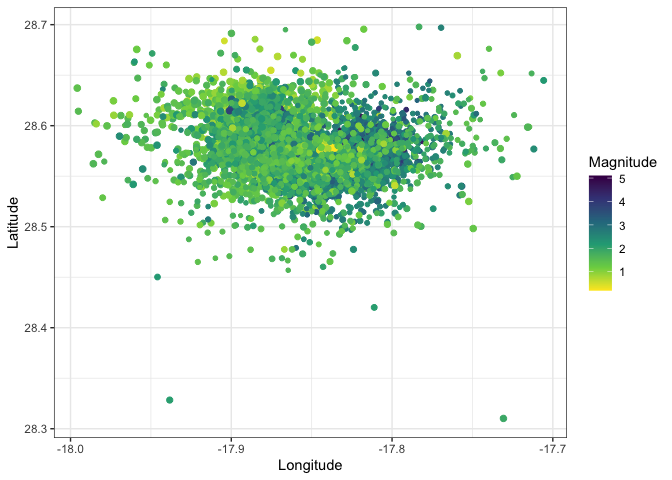
\includegraphics{index_files/figure-latex/notebooks-explore-earthquakes-fig-spatial-plot-output-1.png}

}

\end{figure}%

\textsubscript{Source:
\href{https://kbmcgowan.github.io/play-manuscript/notebooks/explore-earthquakes.qmd.html\#cell-fig-spatial-plot}{Explore
Earthquakes}}

Figure~\ref{fig-spatial-plot} shows the location of recent Earthquakes
on La Palma.

\subsection{Data \& Methods}\label{sec-data-methods}

\subsection{Conclusion}\label{conclusion}

\subsection*{References}\label{references}
\addcontentsline{toc}{subsection}{References}

\phantomsection\label{refs}
\begin{CSLReferences}{1}{0}
\bibitem[\citeproctext]{ref-beddorcoetzeestylermcgowanboland2018}
Beddor, P. S., Coetzee, A. W., Styler, W., McGowan, K. B., \& Boland, J.
E. (2018). The time course of individuals' perception of coarticulatory
information is linked to their production: Implications for sound
change. \emph{Language}, \emph{94}(4), 931--968.

\bibitem[\citeproctext]{ref-beddormcgowanbolandcoetzeebrasher2013}
Beddor, P. S., McGowan, K. B., Boland, J. E., Coetzee, A. W., \&
Brasher, A. (2013). The time course of perception of coarticulation.
\emph{The Journal of the Acoustical Society of America}, \emph{133}(4),
2350--2366.

\bibitem[\citeproctext]{ref-calder2018}
Calder, J. (2018). From {``gay lisp''} to {``fierce queen''}: The
sociophonetics of sexuality's most iconic variable. In K. Hall \& R.
Barrett (Eds.), \emph{The oxford handbook of language and sexuality}
(pp. 1--23).

\bibitem[\citeproctext]{ref-fant1960}
Fant, G. (1960). \emph{Acoustic theory of speech production}. Mouton.

\bibitem[\citeproctext]{ref-kunisakifujisaki1977}
Kunisaki, O., \& Fujisaki, H. (1977). On the influence of context upon
perception of voiceless fricative consonants. \emph{Annual Bulletin},
\emph{11}, 85--91.

\bibitem[\citeproctext]{ref-mackMunson2012b}
Mack, S., \& Munson, B. (2012). The association between/s/quality and
perceived sexual orientation of men's voices: Implicit and explicit
measures. \emph{Journal of Phonetics}, \emph{40}(1), 198--212.

\bibitem[\citeproctext]{ref-MannRepp1980}
Mann, V. A., \& Repp, B. H. (1980). Influence of vocalic context on
perception of the {[}ʃ{]}-{[}s{]} distinction. \emph{Perception \&
Psychophysics}, \emph{28}(3), 213--228.

\bibitem[\citeproctext]{ref-McGurkMacDonald1976}
McGurk, H., \& MacDonald, J. (1976). Hearing lips and seeing voices.
\emph{Nature}, \emph{264}, 746--748.

\bibitem[\citeproctext]{ref-munson2011}
Munson, B. (2011). The influence of actual and imputed talker gender on
fricative perception, revisited (l). \emph{The Journal of the Acoustical
Society of America}, \emph{130}(5), 2631--2634.

\bibitem[\citeproctext]{ref-ohala1984}
Ohala, J. J. (1984). An ethological perspective on common cross-language
utilization of F₀ of voice. \emph{Phonetica}, \emph{41}(1), 1--16.

\bibitem[\citeproctext]{ref-podesvakajino2014}
Podesva, R. J., \& Kajino, S. (2014). Sociophonetics, gender, and
sexuality. \emph{The Handbook of Language, Gender, and Sexuality},
103--122.

\bibitem[\citeproctext]{ref-shadle1991}
Shadle, C. H. (1991). The effect of geometry on source mechanisms of
fricative consonants. \emph{Journal of Phonetics}, \emph{19}(3-4),
409--424.

\bibitem[\citeproctext]{ref-strand1999}
Strand, E. A. (1999). Uncovering the role of gender stereotypes in
speech perception. \emph{Journal of Language and Social Psychology},
\emph{18}(1), 86--100.

\bibitem[\citeproctext]{ref-strandJohnson1996}
Strand, E. A., \& Johnson, K. (1996). Gradient and visual speaker
normalization in the perception of fricatives. \emph{KONVENS}, 14--26.

\bibitem[\citeproctext]{ref-whalen1981}
Whalen, D. H. (1981). Effects of vocalic formant transitions and vowel
quality on the english {[}s{]}--{[}{š}{]} boundary. \emph{The Journal of
the Acoustical Society of America}, \emph{69}(1), 275--282.

\bibitem[\citeproctext]{ref-whalen1984}
Whalen, D. H. (1984). Subcategorical phonetic mismatches slow phonetic
judgments. \emph{Perception \& {Psychophysics}}, \emph{35}, 49--64.

\bibitem[\citeproctext]{ref-whalen1991}
Whalen, D. H. (1991). Perception of the english/s/--/\int{}/distinction
relies on fricative noises and transitions, not on brief spectral
slices. \emph{The Journal of the Acoustical Society of America},
\emph{90}(4), 1776--1785.

\end{CSLReferences}




<div id="criticnav">
<ul>
<li id="markup-button">Markup</li>
<li id="original-button">Original</li>
<li id="edited-button">Edited</li>
</ul>
</div>

<script type="text/javascript">
  function critic() {

      $('.content').addClass('markup');
      $('#markup-button').addClass('active');
      $('ins.break').unwrap();
      $('span.critic.comment').wrap('<span class="popoverc" /></span>');
      $('span.critic.comment').before('&#8225;');
  }

  function original() {
      $('#original-button').addClass('active');
      $('#edited-button').removeClass('active');
      $('#markup-button').removeClass('active');

      $('.content').addClass('original');
      $('.content').removeClass('edited');
      $('.content').removeClass('markup');
  }

  function edited() {
      $('#original-button').removeClass('active');
      $('#edited-button').addClass('active');
      $('#markup-button').removeClass('active');

      $('.content').removeClass('original');
      $('.content').addClass('edited');
      $('.content').removeClass('markup');
  } 

  function markup() {
      $('#original-button').removeClass('active');
      $('#edited-button').removeClass('active');
      $('#markup-button').addClass('active');

      $('.content').removeClass('original');
      $('.content').removeClass('edited');
      $('.content').addClass('markup');
  }

  var o = document.getElementById("original-button");
  var e = document.getElementById("edited-button");
  var m = document.getElementById("markup-button");

  window.onload = critic();
  o.onclick = original;
  e.onclick = edited;
  m.onclick = markup;
</script>



\end{document}
